\chapter[Problem Description]{Problem Description}
\label{ProblemDescription}


% In this section details about the formulation of the Last Mile
% Delivery Drones (LMDD) as a MAPF in a grid and a mathematical model
% of the problem are presented. At the core of MAPF lies the objective
% of crafting collision-free paths for a set of agents, each
% navigating from individual starting points to, respectively, goal
% destinations. As delineated in \citeonline{ijcai2022p0783}, tackling
% this issue generally involves the use of compilation, a notable
% computing technique. This process is defined by the conversion of an
% input instance from its original formalism into a different, usually
% well-established formalism, thereby creating a reduced problem for
% which an efficient solver exists. This reduction is crucial, as it
% essentially simplifies the original problem into a more manageable
% form, optimizing the problem-solving process.

%  The Last Mile Delivery Drones problem can be reduced as a set of
%  tasks for each agent(drone), where each task is described by two
%  tuples $task_i \coloneq \{(x_{\text{start}_i}, y_{\text{start}_i}) ,
%  (x_{\text{goal}_i}, y_{\text{goal}_i})\} ,$ $\forall $ drone $d_i$, with
%  $x,y \in \mathbb{Z}_{\geq 0} $, describing the start position of the drone and
%  the final objective position. In our discretization we make the
%  grid finite, where each axis has bounds, i.e. $x \leq X, y \leq Y$, with
%  $X$ and $Y$ being the bounds of the grid. Our goal is to find paths
%  $P_{d_{i}} \coloneq \{(x_{\text{start}}, y_{\text{start}},
%  t_{\text{begin}} ), (x_{\text{decision}_1}, y_{\text{decision}_1},
%  t_{\text{begin}}+1),(x_{\text{decision}_2}, y_{\text{decision}_2},
%  t_{\text{begin}}+2) \dots, (x_{\text{goal}}, y_{\text{goal}} ,
%  t_{\text{begin}} + | P_{d_i} | ) \} $ for each drone $d_i$ making
%  the path length as short as possible.

% Navigational constraints dictate that each drone's movement is
% restricted to parallel advancements along the grid axes, thus
% excluding the possibility of diagonal traversals to streamline
% pathfinding complexity. Consequently, each drone is limited to four
% principal movements: upward $(x, y+1)$, downward $(x, y-1)$,
% rightward $(x+1, y)$, and leftward $(x-1, y)$ shifts. Formally, a
% position within the grid $(x_1,y_1)$ is adjacent to $(x_2,y_2)$ $\iff
% |x_2-x_1| + |y_2-y_1| = 1$ .

% It is clear how close this formulation is to the MAPF problem. In
% fact, the only difference is now we have a new decision variable,
% the time that each drone starts their flight($t_{\text{begin}}$),
% i.e, the arrival time when the drone takeoff. The analogy with MAPF
% enhances the understanding of the problem and leverages the
% literature of the LMDD problem to a new paradigm.

% There are currently approximates, compilation and AI search based
% solutions to the MAPF problem \cite{ma2019searching}. But there is a
% lack of MILP based formulations for the problem
% \cite{stern2019multi}. Branch Cut and Price \cite{BCPijcai2019} is a
% MILP solution that hybridizes these approaches, using a
% decomposition framework.

% The cited solutions to MAPF are not quite intuitive and leave a hard
% work for generalization. However, in \citeonline{lavalle} it is
% shown the isomorphism(equivalence) between the MAPF and
% multi-commodity minimum cost maximum flow problem. This work let an
% excellent and easy visualization of MAPF problems. In fact, they can
% all be seem as a Network Flow problem. That being said, we propose a
% network-based formulation of the problem.

% The goal of our LMDD formulation is: given an available time $T$,
% minimize the sum of distances of all drones, while allowing drones
% to wait in cells of the grid and choose when they enter at the
% airspace(the grid). Actually, these two additions are what
% differentiates our formulation from standardly MAPFs as
% \citeonline{BCPijcai2019} and \citeonline{lavalle}. Also, the
% proposed LMDD problem has non-weighted distances, what make the
% problem easier then the MAPF itself. As evidenced in
% \ref{graph-modeling} this formulation could be easily addressed if
% modeled as a graph, where our goal is to find the paths that
% generates the minimum flow in the network/graph.

% \section{MAPF as a multi-commodity Network Flow Problem}

% As shown in \citeonline{yu_timeoptimal}, the Multi-Agent Pathfinding
% (MAPF) problem can be transformed into a network flow problem using
% a time-expanded network and multi-commodity flow approach. This
% transformation involves several key steps and concepts, illustrated
% by the figures below.

% \subsection{Time-Expanded Network}

% The first step is to construct a time-expanded network. In this
% representation, each node in the original grid is duplicated for
% each time step, creating a layered network where each layer
% corresponds to a specific time instance. Edges are added to
% represent possible moves between nodes over time, including waiting
% in place. This transformation allows us to model the time dimension
% explicitly within the network.

% \begin{figure}[H]
%     \centering
%     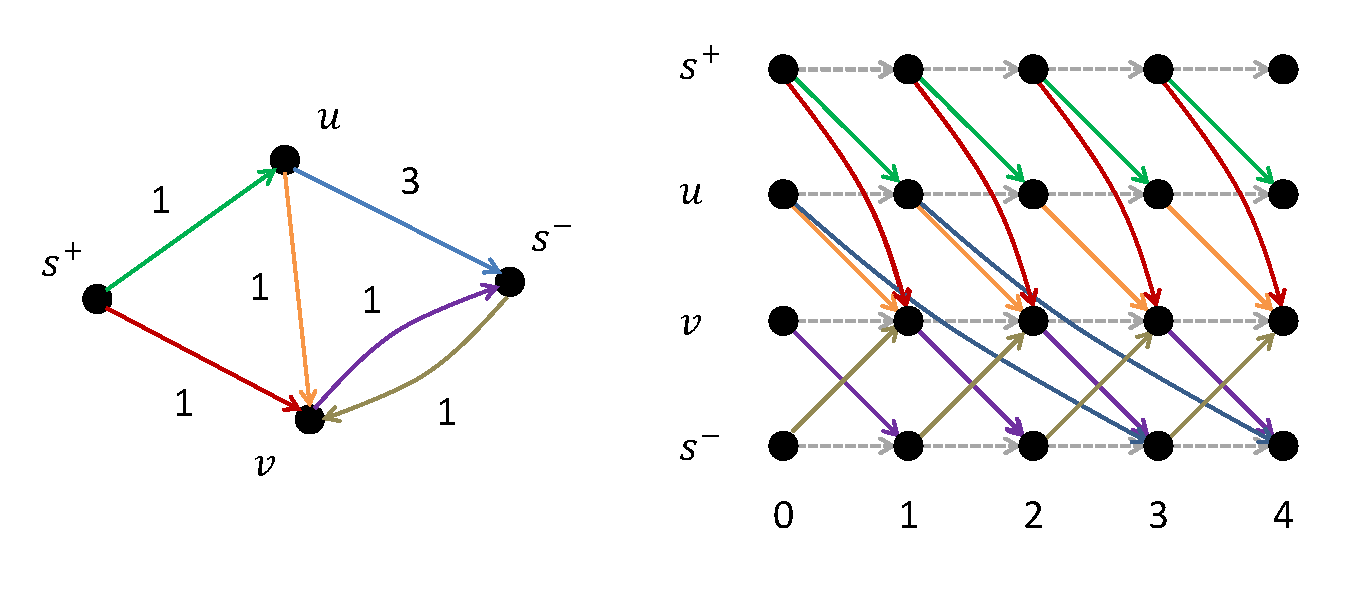
\includegraphics[width=0.8\textwidth]{img/time_extended_net_image.pdf}
%     \caption[Time-expanded network representation]{A time-expanded
%     network representation. Picture sourced from
%     \citeonline{time_optimal_slides}.}
%     \label{fig:time_expanded_network}
% \end{figure}


% \subsection{Multi-Commodity Flow Formulation}

% In this transformed network, the MAPF problem is equivalent to a
% multi-commodity flow problem. Each drone is considered a separate
% commodity that needs to flow from its start node to its goal node
% through the network. The key constraints include ensuring that each
% drone reaches its goal within a given time horizon $T$.

% \begin{figure}[H]
%     \centering
%     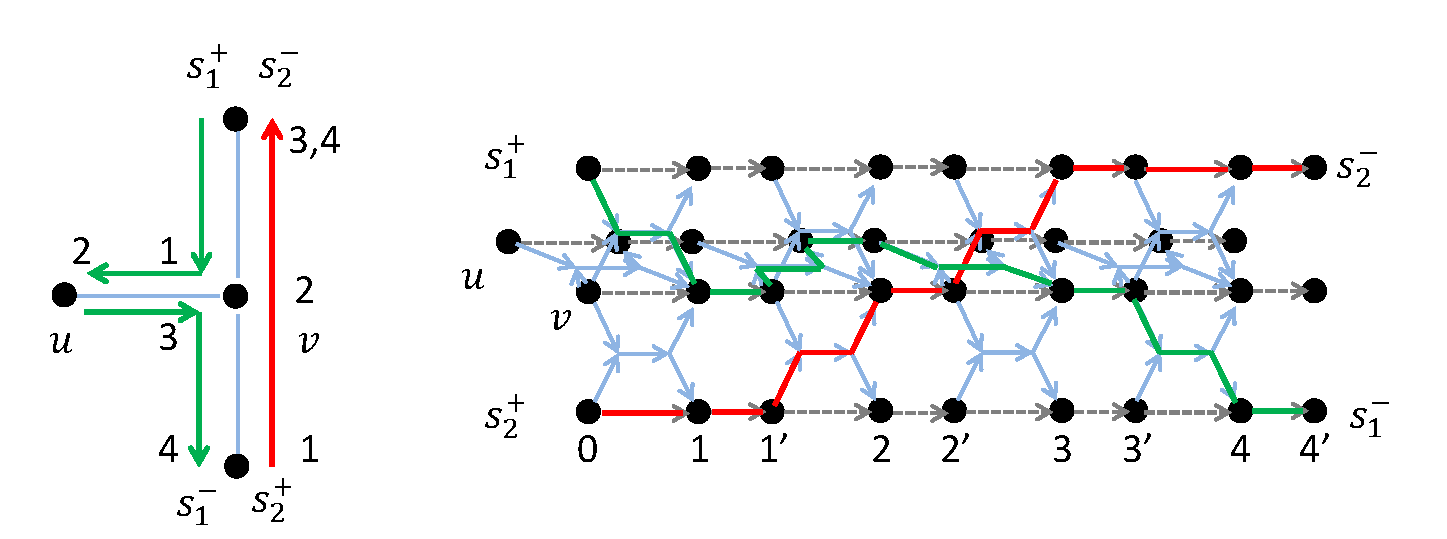
\includegraphics[width=0.8\textwidth]{img/equi_mapf_flow_image.pdf}
%     \caption{Equivalence of MAPF to multi-commodity network flow
%     (sourced from \citeonline{time_optimal_slides})}
%     \label{fig:equi_mapf_flow}
% \end{figure}

% The equivalence between MAPF and multi-commodity network flow is
% fundamental because it allows the application of well-established
% network flow algorithms to solve MAPF problems. By leveraging this
% equivalence, it is possible to find paths for all drones in a
% computationally efficient manner, especially when combined with
% integer linear programming (ILP) techniques.

% This transformation not only provides a clearer visualization of the
% problem but also enhances the ability to apply optimization
% techniques to find solutions. Consequently, it supports the
% development of more efficient algorithms for last-mile delivery
% drones and other applications requiring coordinated multi-agent
% pathfinding.
